\RequirePackage{fix-cm}
\documentclass[smallextended]{svjour3} 
\journalname{Computing}
% Submission version prepared for Computing.

\smartqed  

\usepackage{graphicx}
\usepackage{booktabs} 
\usepackage{amsmath} 
\usepackage{amssymb}
\usepackage{xcolor} 
\usepackage{colortbl} 
\usepackage[numbers,sort&compress,square]{natbib}
\usepackage{algorithm}       
\usepackage{tabularx}      
\usepackage{array}
\usepackage{microtype}
\usepackage{algpseudocode}
\usepackage{placeins}
\newcolumntype{Y}{>{\raggedright\arraybackslash}X}


\begin{document}

\title{Risk-Constrained Selective Answering with Cost-Aware Verification for Scientific RAG}
\titlerunning{Risk-Constrained Selective Answering for Scientific RAG}

\author{Yihan Peng}
\authorrunning{Yihan Peng}

\institute{Yihan Peng \at
Intelligent Science and Technology, Hainan International College, Communication University of China, Lingshui 572400, China \\
\email{202429013035n@mails.cuc.edu.cn}
}

\date{}

\maketitle

\begin{abstract}
Retrieval-augmented generation (RAG) can retrieve relevant scientific passages yet still return low-quality or weakly supported answers. The operational question is when to release an answer and when verification is worth its cost. This paper formulates scientific RAG as risk-constrained selective answering and presents VeriMind, a system that combines structure-aware retrieval with a cost-aware answer-control policy. Candidate answers are ranked using deployment-time features that exclude gold labels and LLM-judge outputs. Low-scoring answers are withheld, high-scoring answers are released directly, and only an uncertain middle region invokes an LLM verifier. Evaluation uses normalized QASPER Answer F1 as a judge-independent outcome and separates model fitting, policy calibration, and held-out testing. On a disjoint 150-question held-out set, the cheap quality score achieved Spearman correlation $0.4137$ with Answer F1 and observed area under the risk--coverage curve (AURC) $0.2915$, compared with $-0.1046$ and $0.3840$ for the legacy trust score. Under a calibration risk budget of $0.55$, the frozen cascade answered 23 questions with mean Answer F1 $0.5046$ and invoked the verifier for 13 questions. This used an estimated 6,811 verifier input tokens, an $88\%$ reduction relative to verifying every naturally answered candidate. Public-benchmark and controlled stress-test analyses further characterize evidence support, abstention, and evaluator sensitivity. The results show that selective answer control is most useful when reported as an explicit quality--coverage--cost operating policy rather than as an unconditional hallucination-elimination claim.
\keywords{Retrieval-Augmented Generation \and Selective Prediction \and Scientific Question Answering \and Risk--Coverage Analysis \and Cost-Aware Verification \and Evidence Control}
\end{abstract}

\section{Introduction}
\label{sec:introduction}

Large language models (LLMs) are increasingly used in scientific question answering, literature analysis, evidence tracing, and decision-support applications. Retrieval-augmented generation (RAG) improves access to external evidence, but retrieval does not by itself determine whether a generated answer is useful enough to release. In a scientific information system, the relevant operational decision is selective: answer when expected quality is adequate, request additional verification when uncertainty is material, and abstain when the available evidence does not support a useful response.

This decision couples three quantities that are often reported separately: answer quality, answer coverage, and verification cost. Always answering maximizes availability but exposes low-quality responses. Always invoking a strong verifier can improve screening but duplicates expensive inference even for easy cases. Aggressive abstention can reduce observed error while making the system unhelpful. A deployable policy must therefore expose an operating point on a quality--coverage--cost frontier rather than optimize any one quantity in isolation.

A methodological complication is that an LLM judge can become entangled with the policy it evaluates. If the same judge score helps decide which answers pass and also defines the reported error event, a low post-gate error rate does not independently establish answer quality. We avoid making that circular comparison the primary evidence. Instead, normalized QASPER Answer F1 supplies a reference-based outcome that is not an input to the deployed policy, while LLM-based faithfulness judgments are retained as secondary diagnostics and as an optional verification signal.

To study this setting, we present VeriMind, a scientific RAG system with structured parsing, adaptive retrieval, and risk-constrained answer control. A cheap quality model uses only response-time information: retrieval similarity, answer--context token coverage, numeric support, length features, question type, and routed granularity. A cost-aware cascade withholds low-scoring answers, directly releases high-scoring answers, and invokes an LLM verifier only for the uncertain middle region. Thresholds are selected on a calibration split under a predeclared selective-risk budget and frozen before evaluation on a disjoint held-out set.

The core contributions of this work are summarized as follows:
\begin{itemize}
    \item \textbf{A risk-constrained scientific RAG formulation:} We cast answer endorsement as selective prediction under an explicit quality--coverage constraint, separating retrieval and generation from the decision to release an answer.

    \item \textbf{A judge-independent quality signal:} We train a lightweight answer-quality ranker from deployment-time features and evaluate it with normalized QASPER Answer F1, risk--coverage curves, and AURC. Gold answers, gold evidence, LLM-judge scores, and the legacy trust score are excluded from its inputs.

    \item \textbf{Cost-aware optional verification:} We introduce a three-way cascade that spends verifier calls only on an uncertain score region and reports verifier call rate and estimated input-token demand alongside answer quality and coverage.

    \item \textbf{Frozen held-out evaluation:} Model fitting, policy calibration, and final testing are separated. The cost-aware policy is selected on a deterministic development/calibration split and evaluated once on a non-overlapping 150-question QASPER set with bootstrap uncertainty intervals.

    \item \textbf{Complementary evidence audits:} QASPER, SciFact, a controlled ten-strategy stress test, cross-judge comparisons, and author-conducted blind audits are used to characterize evidence support and evaluator sensitivity without treating judge-defined error rates as the sole outcome.
\end{itemize}

\section{Related Work}
\label{sec:related_work}

VeriMind intersects scientific question answering, adaptive retrieval, and selective response control. QASPER anchors information-seeking questions in research papers and requires evidence-supported answers \citep{dasigi2021dataset}, making it suitable for studying not only retrieval but also whether a generated answer should be released.

\subsection{Adaptive Retrieval and Generation Control}
RAG augments generation with non-parametric memory \citep{lewis2020retrieval}; REALM and RETRO established retrieval-integrated language modeling \citep{guu2020realm,borgeaud2022improving}. Later systems adapt the post-retrieval path through selective compression, active retrieval, corrective retrieval, or question-complexity routing \citep{xu2023recomp,jiang2023active,yan2024corrective,jeong-etal-2024-adaptive}. Self-RAG couples retrieval control to learned reflection tokens, while HyDE improves dense retrieval through hypothetical documents \citep{asai2023self,gao2022precise}. VeriMind instead separates retrieval routing from a recalibratable release policy and uses multiple index granularities for different evidence needs.

\subsection{Evidence Evaluation and Selective Answering}
Automated RAG evaluation includes judge-based faithfulness, atomic-fact verification, and component-level diagnostics \citep{zheng2023judging,es2024ragas,min2023factscore,saad2023ares,ru2024ragchecker}. These tools primarily evaluate completed outputs. VeriMind converts deployment-time evidence signals into an online answer, verify, or abstain decision. Because judge outputs vary across evaluator families and error types \citep{krishna-etal-2025-fact}, the primary outcome is reference-based Answer F1; judge agreement and author audits remain complementary diagnostics. This decoupled design complements context-faithful generation and source-reliability modeling \citep{zhang-etal-2025-faithfulrag,hwang-etal-2025-retrieval}.

\begin{table*}[t]
\centering
\caption{Architectural comparison between VeriMind and representative RAG frameworks.}
\label{tab:method_comparison}
\footnotesize
\setlength{\tabcolsep}{3pt}
\renewcommand{\arraystretch}{1.18}
\begin{tabularx}{\textwidth}{@{}p{0.16\textwidth}YYYY@{}}
\toprule
\textbf{Method} & \textbf{Routing Strategy} & \textbf{Granularity} & \textbf{Trust Evaluation} & \textbf{Refusal Mechanism} \\ 
\midrule
Vanilla RAG & Static & Fixed-length chunk & None & Forced generation \\
HyDE & Query expansion & Fixed-length chunk & None & Forced generation \\
Self-RAG & On-demand token-level control & Fixed-length chunk & Implicit critique tokens & Soft low-confidence generation \\
CRAG & Retrieval-confidence control & Fixed-length chunk & Limited evaluator with fallback & Soft knowledge bypass \\
\rowcolor{gray!10}
\textbf{VeriMind} & \textbf{Intent-driven} & \textbf{Adaptive three-space indexing} & \textbf{Cheap score + optional verifier} & \textbf{Answer, verify, or abstain} \\
\bottomrule
\end{tabularx}
\end{table*}

As compared in Table~\ref{tab:method_comparison}, prior RAG variants typically focus on retrieval adaptation, self-reflective generation control, or post-hoc factual evaluation. VeriMind combines multi-granularity routing with a risk-constrained response policy and optional verification. Its target is an explicit quality--coverage--cost operating point for knowledge-intensive question answering.

\section{System Design of the Selective Scientific RAG System}
\label{sec:methodology}

\begin{figure*}[t]
\centering
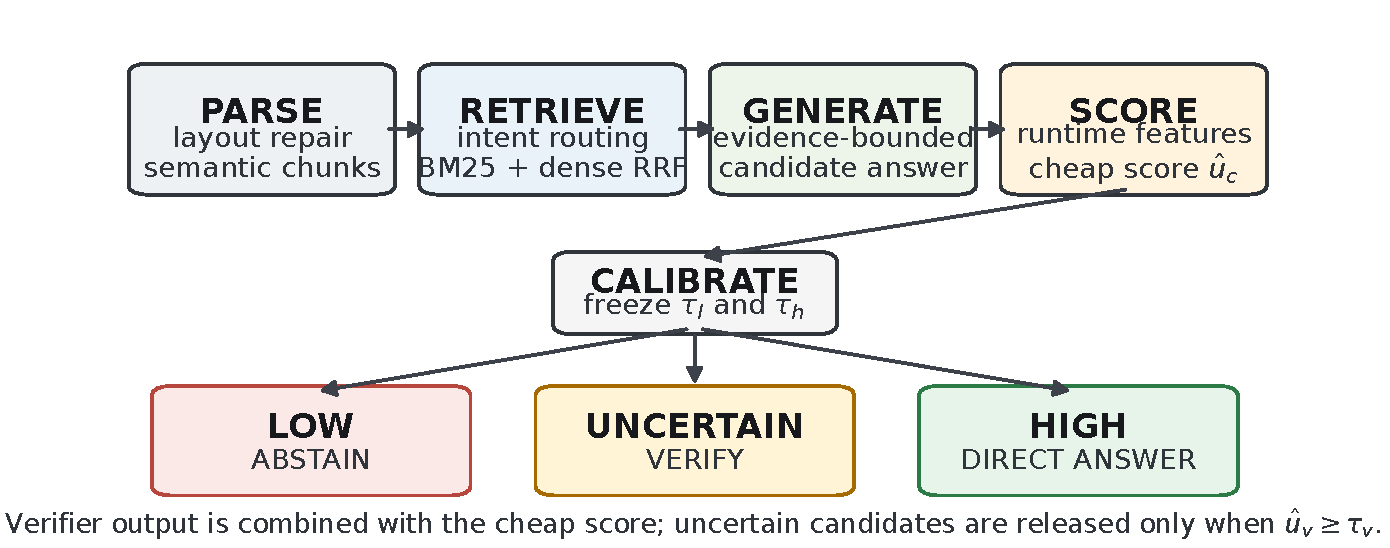
\includegraphics[width=\textwidth]{Fig1_architecture.pdf}
\caption{Risk-constrained scientific RAG architecture. Deployment-time features produce a cheap quality score; low-score candidates are withheld, high-score candidates are released directly, and uncertain candidates invoke an optional verifier before release. Thresholds are frozen after calibration.}
\label{fig:architecture}
\end{figure*}

VeriMind spans structure-aware preprocessing, intent-driven retrieval routing, candidate generation, and risk-constrained response control.

\subsection{Structural Markdown Parsing and Heuristic Layout Analysis}
\label{sec:structural_parsing}

Academic PDFs contain multi-column layouts, marginal metadata, headings, tables, and cross-page continuations that are easily corrupted by plain-text extraction. VeriMind reconstructs reading order from block coordinates, filters recurrent headers and footers using relative page positions, and maps typography to hierarchical Markdown. Chunk boundaries are then restricted to headings and paragraph boundaries so that the three retrieval spaces receive structurally coherent text rather than arbitrary flattened spans.

\subsection{Intent-Driven Multi-Granularity Routing}
\label{sec:routing}

Conventional RAG systems face a ``granularity dilemma'': fine-grained chunks isolate entities and numerical metrics but can remove their surrounding context. Coarse-grained chunks preserve narrative flow but add retrieval noise that dilutes precise matches. VeriMind therefore uses three parallel vector spaces: $\mathcal{G}_{detail}$, $\mathcal{G}_{concept}$, and $\mathcal{G}_{context}$. Their chunk sizes, overlap rates, and retrieval roles are detailed in Table~\ref{tab:granularity_params}.

\begin{table*}[t]
\centering
\caption{Parameterization and Academic Rationale of the Index Spaces}
\label{tab:granularity_params}
\resizebox{\textwidth}{!}{
\begin{tabular}{@{}lcccp{6cm}@{}}
\toprule
\textbf{Intent Space} & \textbf{Chunk Size} & \textbf{Overlap} & \textbf{Target Queries} & \textbf{Academic Rationale} \\ \midrule
$\mathcal{G}_{detail}$ (Micro) & 128 tokens & 0\% & Exact metrics, hyper-parameters & Minimizes semantic dilution for factual pinpointing; overlap is 0\% to prevent redundant micro-hits. \\
$\mathcal{G}_{concept}$ (Standard)& 512 tokens & 15\% & Definitions, methodology steps & Balances entity representation with local context; standard setting for most semantic retrievers. \\
$\mathcal{G}_{context}$ (Macro) & 1024 tokens & 20\% & Multi-hop reasoning, summaries & Preserves long-range logical flow across paragraphs; high overlap prevents critical evidence severance. \\ \bottomrule
\end{tabular}%
}
\end{table*}

The intent-driven router ($\mathcal{F}_{router}$) maps each query to one of the three retrieval spaces using a constrained language-model classifier. Unlike static length rules, this decision uses the semantic evidence need expressed by the query. The routing logic is formalized in Algorithm~\ref{alg:routing}.

\begin{algorithm}[htbp]
\caption{Intent-Driven Multi-Granularity Routing}
\label{alg:routing}
\begin{algorithmic}[1]
\Require User query $q$, Few-shot prompt template $\mathcal{P}$, LLM generator $\mathcal{M}$
\Ensure The optimal retrieved context $C_{opt}$
\State Construct routing prompt: $p_{route} \gets \mathcal{P} \oplus q$
\State Intent $I \gets \mathcal{M}(p_{route})$ \Comment{LLM deduces latent cognitive demand}
\If{$I$ == "DETAIL"}
    \State $\mathcal{G}_{target} \gets \mathcal{G}_{detail}$ \Comment{128-token space}
\ElsIf{$I$ == "CONTEXT"}
    \State $\mathcal{G}_{target} \gets \mathcal{G}_{context}$ \Comment{1024-token space}
\Else
    \State $\mathcal{G}_{target} \gets \mathcal{G}_{concept}$ \Comment{Fallback to 512-token standard space}
\EndIf
\State $C_{opt} \gets \text{Top-K-Retrieval}(q, \mathcal{G}_{target})$
\State \textbf{return} $C_{opt}$
\end{algorithmic}
\end{algorithm}

To overcome the semantic mismatch inherent in purely dense retrieval systems, VeriMind implements a multi-granularity hybrid retrieval mechanism. Initially, a sparse lexical retriever based on the classical BM25 algorithm \citep{robertson2009probabilistic} executes a keyword-centric extraction to ensure exact-match preservation for domain-specific terminologies. Concurrently, a dense retriever utilizing the \texttt{text-embedding-v1} architecture maps the query into a high-dimensional continuous neural vector space, akin to the Dense Passage Retrieval (DPR) paradigm \citep{karpukhin2020dense}. The outputs are subsequently fused utilizing Reciprocal Rank Fusion (RRF).

The router uses a fixed few-shot prompt and is constrained to output exactly one of \texttt{DETAIL}, \texttt{CONCEPT}, or \texttt{CONTEXT}. It performs a single classification step rather than an iterative reasoning loop. The same prompt template is held fixed across compared routing conditions.

\subsection{Risk-Constrained Selective Answer Control}
\label{sec:trust_scoring}

Let $q$ denote a question, $C$ its retrieved context, and $a$ the generated candidate answer. VeriMind separates candidate generation from answer endorsement. The primary policy estimates answer utility with a cheap score $\hat{u}_{c}$ and reserves LLM-based verification for candidates near the decision boundary. This design avoids paying verifier cost for every generated answer and allows the operating policy to be calibrated against an explicit selective-risk budget.

\paragraph{Deployment-time quality features.}
The cheap feature vector is
\begin{equation}
x(q,a,C) = [s_{ret}, c_{tok}, c_{num}, \ell_a, \ell_q, t_q, g_q],
\label{eq:cheap_features}
\end{equation}
where $s_{ret}$ is average retrieval similarity, $c_{tok}$ is unique answer-token coverage in the retrieved context, $c_{num}$ measures whether numeric claims in the answer occur in the context, $\ell_a$ and $\ell_q$ are answer and question lengths, $t_q$ is a deterministic lexical question type, and $g_q$ is the routed retrieval granularity. A ridge regressor estimates $\hat{u}_{c}=f_{\theta}(x)\in[0,1]$. The model inputs exclude reference answers, annotated evidence, hallucination labels, LLM-judge scores, and the legacy trust score.

\paragraph{Optional verifier.}
For candidates routed to verification, an independent LLM scores answer support against the retrieved context \citep{zheng2023judging}. A second ridge model combines the cheap score and normalized verifier score to obtain $\hat{u}_{v}$. The verifier is therefore a policy input for uncertain cases, not the definition of the primary evaluation outcome. Answer quality is evaluated separately with normalized QASPER Answer F1.

\paragraph{Three-way cascade.}
For frozen thresholds $\tau_l$, $\tau_h$, and $\tau_v$, the policy is
\begin{equation}
\pi(q,a,C)=
\begin{cases}
\textsc{Abstain}, & \hat{u}_{c}<\tau_l,\\
\textsc{Verify}, & \tau_l\leq\hat{u}_{c}<\tau_h,\\
\textsc{Answer}, & \hat{u}_{c}\geq\tau_h.
\end{cases}
\label{eq:cascade_policy}
\end{equation}
Candidates in the middle region are released only when $\hat{u}_{v}\geq\tau_v$. Thresholds are selected on calibration data by maximizing answer coverage subject to selective risk $R(\pi)\leq\epsilon$; ties prefer fewer verifier calls and then lower observed risk. If no policy satisfies a requested budget, the procedure reports the lowest-risk observed policy as infeasible rather than silently relaxing the constraint.

Algorithm~\ref{alg:gating} summarizes the resulting response policy.

\begin{algorithm}[htbp]
\caption{Cost-Aware Selective Answering Protocol}
\label{alg:gating}
\begin{algorithmic}[1]
\Require Query $q$, context $C$, candidate $a$, cheap model $f_{\theta}$, optional verifier $\mathcal{M}_{judge}$, thresholds $(\tau_l,\tau_h,\tau_v)$
\Ensure Final answer $A_{final}$ and decision $S$
\State Extract deployment-time features $x(q,a,C)$
\State Predict cheap utility $\hat{u}_{c}\gets f_{\theta}(x)$
\If{$\hat{u}_{c}<\tau_l$}
    \State $S\gets\textsc{Abstain}$; $A_{final}\gets\text{``Information not found.''}$
\ElsIf{$\hat{u}_{c}\geq\tau_h$}
    \State $S\gets\textsc{Answer-Direct}$; $A_{final}\gets a$
\Else
    \State Obtain verifier score $s_v\gets\mathcal{M}_{judge}(q,a,C)$
    \State Predict verified utility $\hat{u}_{v}\gets f_v(\hat{u}_{c},s_v)$
    \If{$\hat{u}_{v}\geq\tau_v$}
        \State $S\gets\textsc{Answer-Verified}$; $A_{final}\gets a$
    \Else
        \State $S\gets\textsc{Abstain-Verified}$; $A_{final}\gets\text{``Information not found.''}$
    \EndIf
\EndIf
\State \textbf{return} $A_{final}, S$
\end{algorithmic}
\end{algorithm}

The original implementation used a scalar legacy score that linearly combined calibrated retrieval similarity and an LLM faithfulness score. We retain that score as a comparator in the ranking analysis, but not as the principal quality estimator, because its LLM component also informed the earlier automated hallucination labels. This distinction separates policy evaluation from evaluator agreement.

\paragraph{Frozen Three-Judge Gate V2 Audit Policy.}
The empirical audit also includes a frozen three-judge Gate V2 rule. It is used only for comparison with the author-blind evidence audit and does not select the cheap model or the cost-aware cascade. Gate V2 rejects an answer when at least two judges mark it unsupported, warns when exactly one judge marks it unsupported or any judge is uncertain, and otherwise accepts it.

\section{Evaluation Datasets}
\label{sec:dataset}

\subsection{QASPER Public Benchmark}
\label{subsec:qasper_dataset}

QASPER is a public information-seeking question-answering dataset anchored in full research papers \citep{dasigi2021dataset}. It is particularly suitable for this study because questions require evidence distributed across scientific-paper sections and include both answerable and unanswerable cases. We construct a deterministic evaluation subset of 300 validation questions spanning 182 papers, with 240 answerable and 60 unanswerable questions. Selection is based on a fixed hash of the public question identifier, targeting a 20\% unanswerable share without model-dependent filtering. For each question, retrieval is restricted to its associated paper, following QASPER's single-document task definition. The paper is nevertheless chunked and indexed at multiple granularities, so the experiment tests evidence localization, answer generation, and selective response control rather than global document identification.

\subsection{VeriMind-Bench as a Controlled Stress Test}
\label{subsec:verimind_bench}

Generalized benchmarks do not fully expose adversarial premises, recent-literature leakage, and controlled evidence-absence cases. We therefore retain VeriMind-Bench as a complementary stress test rather than the sole empirical basis of the study. The dataset is designed to assess hallucination mitigation \citep{ji2023survey} under recent scientific literature and explicit boundary cases.

\subsubsection{Knowledge Corpus Curation and Leakage Mitigation}
\label{subsec:corpus_curation}
A common methodological limitation in evaluating neural Language Models is \textit{Pre-training Data Leakage}, a condition where models answer queries correctly by retrieving information from their latent pre-training weights rather than through active RAG retrieval. To rigorously minimize this risk, the knowledge corpus of VeriMind-Bench is assembled exclusively from 118 recent top-tier Artificial Intelligence conference papers (e.g., ACL, NeurIPS, ICLR) published after 2023. 

By isolating literature that discusses recent sub-domains---specifically LLM reasoning, RAG architectures, long-context evaluation, and alignment---the dataset encourages foundation models to rely on dynamically retrieved context. This corpus constitutes approximately 1,200 pages of academic text.

\subsubsection{Taxonomy of Question Categories}
\label{subsec:qa_taxonomy}
VeriMind-Bench is formulated as a dense challenge set comprising 300 zero-shot queries. To systematically evaluate the boundary conditions of the RAG framework, the queries are stratified into four distinct cognitive dimensions:

\begin{enumerate}
    \item \textbf{Reasoning QA (120 queries):} Requires the model to deduce causal relationships, compare algorithmic parameters, or synthesize methodological rationales scattered across paragraphs.
    \item \textbf{Factual QA (80 queries):} Demands the precise extraction of exact numerical metrics, hyper-parameters, or algorithmic naming conventions.
    \item \textbf{Multi-hop QA (60 queries):} Necessitates iterative retrieval and logical bridging across multiple independent document chunks to formulate a conclusion.
    \item \textbf{Adversarial Trap-QA (40 queries):} Deliberately injected with fabricated premises or non-existent entities (e.g., querying the ``BLEU score of a model on an unmentioned dataset''). These queries serve as a controlled stress test for the system's defensive rejection mechanisms.
\end{enumerate}

The statistical distribution of the dataset corpus is detailed in Table~\ref{tab:dataset_stats}.

\begin{table*}[t]
\centering
\caption{Statistical Distribution of the VeriMind-Bench Dataset across AI Sub-domains}
\label{tab:dataset_stats}
\renewcommand{\arraystretch}{1.2}
\resizebox{\textwidth}{!}{
\begin{tabular}{@{}lccccc@{}}
\toprule
\textbf{Sub-domain Category} & \textbf{Papers} & \textbf{Reasoning QA} & \textbf{Factual QA} & \textbf{Multi-hop QA} & \textbf{Adversarial Trap-QA} \\
\midrule
RAG Optimization \& Architecture & 42 & 45 & 30 & 20 & 15 \\
LLM Reasoning \& Tool Use & 38 & 40 & 25 & 20 & 10 \\
Long-Context Evaluation & 20 & 20 & 15 & 10 & 8 \\
Trustworthiness \& Alignment & 18 & 15 & 10 & 10 & 7 \\
\midrule
\textbf{Aggregate Total} & \textbf{118} & \textbf{120} & \textbf{80} & \textbf{60} & \textbf{40} \\
\bottomrule
\end{tabular}%
}
\end{table*}

\subsubsection{Generation Pipeline and Quality Control}
\label{subsec:quality_control}
To ensure high-fidelity ground truths, the query generation pipeline integrates both automated synthesis and human verification. Initially, a section-aware chunking algorithm partitions the 118 papers into semantically complete segments. Candidate QA pairs are then generated via an LLM prompted for the specific cognitive intents outlined in Section~\ref{subsec:qa_taxonomy}. 

Subsequently, an automatic deduplication mechanism computes semantic embeddings for all generated queries, filtering out redundant questions based on cosine similarity thresholds. The selected questions, reference answers, and evaluation records were manually audited by the author under a predefined annotation protocol. These checks are used as author-conducted audit evidence rather than as third-party annotations.

To improve the traceability of the evaluation process, we separately maintained blind audit sheets for QASPER answer-level checks. The audit sheets hid gate decisions and model-judge labels during labeling, and the completed labels were merged back only after the audit step. This protocol supports error analysis and calibration checks while avoiding overstatement of the human-validation evidence.

\section{Experimental Setup}
\label{sec:experimental_setup}

The evaluation separates reference-based selective answering from secondary automated-faithfulness diagnostics.

\subsection{Baseline Models and Comparative Paradigms}
\label{subsec:baselines}
The baselines isolate retrieval, context, self-critique, and system-component effects:

\begin{enumerate}
    \item \textbf{Naive RAG} uses fixed 512-token chunks and static Top-$K$ dense retrieval without post-generation verification \citep{lewis2020retrieval}.
    \item \textbf{HyDE} retrieves with a generated hypothetical document \citep{gao2022precise}.
    \item \textbf{Self-RAG-style prompting} adds retrieval-awareness and self-critique instructions but does not use the official fine-tuned checkpoint \citep{asai2023self}.
    \item \textbf{Long-Context LLM} receives concatenated top-ranked sections within the model context limit.
    \item \textbf{Internal ablations} disable routing, the legacy scalar gate, or structure-aware parsing.
\end{enumerate}
All ten stress-test strategies use the same 300-question benchmark schema.

\subsection{Public-Benchmark, Annotator, and Heterogeneous Robustness Protocol}
\label{subsec:ood_setup}
The robustness protocol combines public held-out evaluation, blind author audits, and heterogeneous evaluators.

\begin{itemize}
    \item \textbf{QASPER:} A deterministic 300-question subset supports development; a non-overlapping 150-question subset is held out. All methods retrieve Top-$K=3$ passages from the associated paper. Normalized Answer F1 is primary; judge labels are secondary.

    \item \textbf{Frozen policy:} The 300 development questions are split into 200 fitting and 100 calibration questions, stratified by answerability. Budgets $\epsilon\in\{0.45,0.50,0.55,0.60\}$ are fixed before the 150-question held-out evaluation; $\epsilon=0.55$ is the strictest calibration-feasible cascade setting.

    \item \textbf{Additional diagnostics:} SciFact tests transfer of retrieval and legacy screening. Blind author audits cover 149 development answers and 96 naturally answered held-out cases. Qwen-Plus, GLM-4.5-Air, and DeepSeek-V3.2 provide complete three-judge coverage for 3,000 stress-test outputs; heterogeneous generator--judge pairs test evaluator sensitivity.

\end{itemize}

\subsection{Comprehensive Evaluation Metrics}
\label{subsec:metrics}
System performance is quantified across answer quality, selective risk, retrieval, and operational cost:

\begin{enumerate}
    \item \textbf{Normalized QASPER Answer F1:} Uses the official-style normalized token overlap between a generated answer and the best matching reference answer. This reference-based outcome is not used as a deployment feature.
    \item \textbf{Selective Risk and Coverage:} For the accepted set $\mathcal{A}_{\pi}$ under policy $\pi$, we define
    \begin{equation}
    R(\pi)=1-\frac{1}{|\mathcal{A}_{\pi}|}\sum_{i\in\mathcal{A}_{\pi}}\mathrm{AnswerF1}_i,
    \qquad
    C(\pi)=\frac{|\mathcal{A}_{\pi}|}{N}.
    \label{eq:selective_risk}
    \end{equation}
    Risk--coverage ranking is summarized by observed AURC; lower values indicate better concentration of high-quality answers at early coverage.
    \item \textbf{Verification Cost:} We report verifier call rate and estimated verifier input tokens. Token demand is approximated as total verifier-input characters divided by four and is used only for relative offline comparison; it is not measured API usage, latency, or monetary cost.
    \item \textbf{Secondary metrics:} ROUGE-L and Exact Match measure reference overlap; HR@K measures retrieval of annotated evidence; raw and passed-hallucination events record unsupported outputs before and after screening; answer coverage is the fraction of questions receiving a non-abstaining response.
\end{enumerate}

\subsection{Statistical Significance Testing Methodology}
\label{subsec:statistics}
Paired hallucination events are compared with McNemar's test \citep{mcnemar1947note}; binomial rates use exact or Wilson intervals as appropriate. Cohen's and Fleiss' $\kappa$ quantify evaluator agreement \citep{cohen1960coefficient}, Fisher's exact test handles sparse audit tables, and Cohen's $h$ summarizes effect size. Frozen-policy uncertainty is estimated with percentile bootstrap intervals.

\subsection{Implementation Details and Policy Calibration}
\label{subsec:implementation}
The QASPER generator outputs are fixed before selective-policy analysis. The cheap quality model is a deterministic ridge-regression pipeline with standardized numeric features and one-hot encoded categorical features. Ridge penalties are selected from $\{0.01,0.1,1,10,100\}$ by five-fold cross-validation on the fitting split. The optional verified model is another ridge regressor whose inputs are the cheap score and normalized LLM faithfulness score. Scores are clipped to $[0,1]$ only after prediction.

Policy thresholds are searched over deciles of the calibration-score distributions. For each risk budget, the selected policy maximizes calibration coverage subject to Eq.~\ref{eq:selective_risk}; ties prefer fewer verifier calls and then lower risk. The held-out labels do not participate in model fitting, threshold selection, or fallback handling. Bootstrap intervals use 2,000 held-out resamples with seed 20260918 and keep every selected policy frozen.

The original retrieval and stress-test experiments use the previously reported generator, judge, embedding, and Top-$K$ configurations. They are retained to describe the retrieval system and evaluator sensitivity, whereas the selective-policy experiment supplies the primary answer-quality and cost analysis.

\paragraph{AI-assisted research workflow.} AI-assisted tools supported language editing, code implementation, experiment orchestration, and result summarization under author supervision. They were not treated as sources of scientific claims; the author verified the analyses, manuscript, and reported results and assumes full responsibility for the work.

\begin{table}[htbp]
\centering
\caption{Selective-policy configuration for QASPER}
\label{tab:exp_setup}
\renewcommand{\arraystretch}{1.2}
\resizebox{\columnwidth}{!}{%
\begin{tabular}{@{}ll@{}}
\toprule
\textbf{Component / Parameter} & \textbf{Configuration Value} \\
\midrule
Development / calibration / held-out & 200 / 100 / 150 questions \\
Cheap model & Standardization + one-hot encoding + ridge regression \\
Verified model & Ridge regression over cheap and verifier scores \\
Ridge penalty grid & $\{0.01,0.1,1,10,100\}$ \\
Risk budgets $\epsilon$ & $\{0.45,0.50,0.55,0.60\}$ \\
Policy-search grid & Score-distribution deciles \\
Bootstrap & 2,000 resamples; seed 20260918 \\
\bottomrule
\end{tabular}%
}
\end{table}

\section{Selective Answering and Reliability Evaluation Results}
\label{sec:results}

\subsection{Judge-Independent Selective Quality on QASPER}
\label{subsec:qasper_results}

We first test whether answer quality can be ranked without using gold information or LLM-judge outputs as policy inputs. Table~\ref{tab:qasper_ranking} reports performance on the disjoint 150-question held-out set. The generator produced 96 non-abstaining candidate answers. The cheap quality score attained Spearman correlation $0.4137$ with normalized Answer F1 and observed AURC $0.2915$. In contrast, retrieval similarity and the legacy trust score were negatively correlated with Answer F1. The cheap score also improved observed AURC over the legacy trust score by $0.0925$; a 5,000-resample paired bootstrap estimated a 95\% interval of $[0.0281,0.1569]$ for this AURC reduction.

\begin{table}[htbp]
\centering
\caption{Held-out ranking of QASPER candidate-answer quality. AURC is computed over the observed candidate-answer coverage range; lower is better.}
\label{tab:qasper_ranking}
\renewcommand{\arraystretch}{1.12}
\small
\begin{tabular}{@{}lrr@{}}
\toprule
\textbf{Deployment score} & \textbf{Spearman with Answer F1} & \textbf{Observed AURC} \\
\midrule
\rowcolor{gray!10}
\textbf{Cheap quality score} & \textbf{0.4137} & \textbf{0.2915} \\
LLM faithfulness score & 0.0464 & 0.3320 \\
Legacy trust score & $-0.1046$ & 0.3840 \\
Retrieval similarity & $-0.2099$ & 0.3932 \\
\bottomrule
\end{tabular}
\end{table}

We next evaluate frozen answer-control policies. Table~\ref{tab:qasper_cost_policy} focuses on the predeclared risk budget $\epsilon=0.55$, the strictest requested budget for which the cascade was feasible on the calibration split. On held-out data, the cascade accepted 23 of 150 questions with mean Answer F1 $0.5046$ and selective risk $0.4954$. It invoked the verifier for 13 questions ($8.67\%$ of the held-out set), corresponding to 6,811 estimated verifier input tokens. Verifying every naturally answered candidate required 56,777 estimated input tokens. The cascade therefore reduced estimated verifier input demand by $88\%$ while attaining nearly twice the held-out coverage of the threshold selected for Always Verify ($15.33\%$ versus $8.00\%$).

\begin{table}[htbp]
\centering
\caption{Frozen held-out policies at calibration risk budget $\epsilon=0.55$. $N$ is the number accepted; ``Cal.'' records calibration feasibility. Held-out risk is reported without threshold reselection.}
\label{tab:qasper_cost_policy}
\renewcommand{\arraystretch}{1.12}
\scriptsize
\setlength{\tabcolsep}{2.2pt}
\begin{tabular}{@{}lrrrrrr@{}}
\toprule
\textbf{Policy} & \textbf{$N$} & \textbf{Coverage} & \textbf{F1} & \textbf{Risk} & \textbf{Verify} & \textbf{Cal.} \\
\midrule
No Gate & 96 & 64.00\% & 0.4362 & 0.5638 & 0.00\% & No \\
Cheap Only & 24 & 16.00\% & 0.5236 & 0.4764 & 0.00\% & No \\
Always Verify & 12 & 8.00\% & 0.5898 & 0.4102 & 64.00\% & No \\
\rowcolor{gray!10}
\textbf{Cost-Aware Cascade} & \textbf{23} & \textbf{15.33\%} & \textbf{0.5046} & \textbf{0.4954} & \textbf{8.67\%} & \textbf{Yes} \\
\bottomrule
\end{tabular}
\end{table}

The bootstrap intervals are intentionally reported as uncertainty rather than as significance claims. For the cascade, the 95\% intervals were $[10.00\%,21.33\%]$ for coverage and $[0.3567,0.6460]$ for selective risk. For Always Verify, the corresponding intervals were $[4.00\%,12.67\%]$ and $[0.2068,0.6182]$. The overlap indicates that the present held-out sample supports a concrete operating-point comparison, not a claim that the cascade has uniformly lower risk than always-on verification. Its demonstrated advantage is targeted verifier use at higher coverage under the policy selected by the calibration constraint.

\begin{figure*}[htbp]
\centering
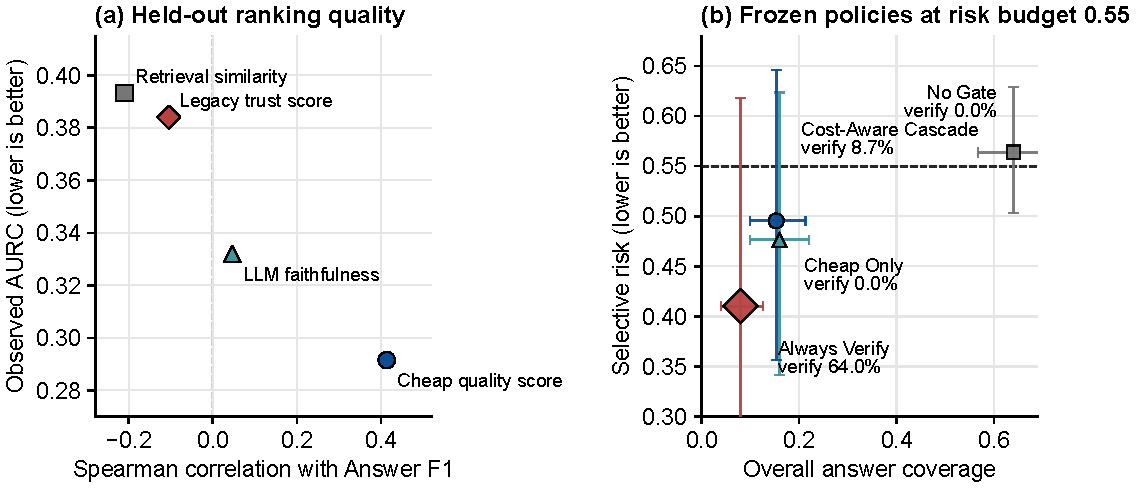
\includegraphics[width=\textwidth]{Fig13_selective_cost_tradeoff.pdf}
\caption{Judge-independent selective quality and frozen policy behavior on held-out QASPER. (a) The cheap deployment score ranks normalized Answer F1 more effectively than individual retrieval or LLM-judge scores. (b) At calibration risk budget $\epsilon=0.55$, the cost-aware cascade concentrates verifier calls in the uncertain region. Error bars are 95\% percentile bootstrap intervals from 2,000 frozen-policy resamples; token demand is analyzed separately because it is an offline estimate.}
\label{fig:qasper_selective_cost}
\end{figure*}
\FloatBarrier

\subsection{Automated Faithfulness Diagnostics on QASPER}

Table~\ref{tab:qasper_results} retains the original LLM-judge faithfulness analysis as a secondary diagnostic. Under this evaluator, VeriMind produced one passed event among 133 accepted answers ($0.75\%$, 95\% Wilson CI: $0.13\%$--$4.14\%$). Vanilla RAG produced 22 among 147 ($14.97\%$), while HyDE produced 13 among 143 ($9.09\%$). Paired McNemar tests yielded $p<10^{-6}$ against Vanilla RAG and $p=4.88\times10^{-4}$ against HyDE. These tests characterize differences under the fixed automated evaluator; they do not replace the judge-independent Answer F1 analysis above.

\begin{table}[htbp]
\centering
\caption{QASPER public-benchmark results on 300 questions. Passed hallucinations are reported as events among accepted answers; conditional ROUGE-L is computed over accepted, answerable questions.}
\label{tab:qasper_results}
\renewcommand{\arraystretch}{1.15}
\small
\setlength{\tabcolsep}{6pt}
\textbf{Safety and coverage.}\\[2pt]
\begin{tabular}{@{}lccc@{}}
\toprule
\textbf{Strategy} & \textbf{Passed / Accepted} & \textbf{Passed Rate} & \textbf{Coverage} \\
\midrule
Vanilla RAG & 22 / 147 & 14.97\% & 49.00\% \\
HyDE & 13 / 143 & 9.09\% & 47.67\% \\
\rowcolor{gray!10}
\textbf{VeriMind Full} & \textbf{1 / 133} & \textbf{0.75\%} & \textbf{44.33\%} \\
VeriMind No Gating & 19 / 149 & 12.75\% & 49.67\% \\
VeriMind No Routing & 1 / 128 & 0.78\% & 42.67\% \\
No Structure & 0 / 102 & 0.00\% & 34.00\% \\
\bottomrule
\end{tabular}

\vspace{0.45em}
\textbf{Accepted-answer utility.}\\[2pt]
\begin{tabular}{@{}lcc@{}}
\toprule
\textbf{Strategy} & \textbf{Answerable Coverage} & \textbf{Cond. ROUGE-L} \\
\midrule
Vanilla RAG & 57.50\% & 0.4242 \\
HyDE & 55.42\% & 0.3915 \\
\rowcolor{gray!10}
\textbf{VeriMind Full} & \textbf{52.08\%} & \textbf{0.3995} \\
VeriMind No Gating & 58.33\% & 0.4186 \\
VeriMind No Routing & 50.00\% & 0.3926 \\
No Structure & 39.17\% & 0.4429 \\
\bottomrule
\end{tabular}
\end{table}

Under the fixed automated evaluator, removing the legacy gate increases accepted coverage from $44.33\%$ to $49.67\%$ and changes passed events from 1 to 19 ($12.75\%$; exact McNemar $p=7.63\times10^{-6}$). Because the judge score contributes to both the legacy gate and this diagnostic label, this comparison demonstrates the behavior of that screening rule rather than independent causal evidence of answer quality. The reference-based selective-risk experiment provides the primary evaluation of answer endorsement. Routing and structure-aware parsing remain retrieval-side ablations: disabling routing reduces overall coverage from $44.33\%$ to $42.67\%$, while removing structure-aware parsing lowers coverage to $34.00\%$ under the legacy gate.

\subsection{Author Audit and Held-out Gate V2 Validation}
\label{subsec:human_validation}
Author-blind audit sheets contained only the question, retrieved context, generated answer, and empty label fields; gate decisions, judge labels, item identifiers, and gold answers were hidden.

The development audit covered all 149 No-Gating answers: 141 supported, 5 unsupported, and 3 uncertain. The original scalar gate caught 1 of 5 unsupported answers and falsely rejected 16 supported answers, motivating its replacement as the primary release signal.

The non-overlapping 150-question held-out set yielded 96 No-Gating answers, all audited before comparison with frozen Gate V2. Gate V2 rejects when at least two judges report unsupported evidence and warns on one unsupported or any uncertain vote.

\begin{table}[H]
\centering
\caption{Held-out QASPER author audit of frozen Gate V2 decisions. Metrics are computed on the 96 No-Gating answers that entered the author-blind audit; overall coverage uses the 150-question held-out denominator.}
\label{tab:heldout_gate_v2_audit}
\renewcommand{\arraystretch}{1.15}
\resizebox{\textwidth}{!}{%
\begin{tabular}{@{}lccccccc@{}}
\toprule
\textbf{Policy} & \textbf{TP} & \textbf{FP} & \textbf{FN} & \textbf{TN} & \textbf{False Rejection} & \textbf{Overall Coverage} & \textbf{Fisher $p$} \\
\midrule
Current scalar gate & 1 & 12 & 0 & 83 & 12.63\% & 55.33\% & 0.1354 \\
\rowcolor{gray!10}
\textbf{Gate V2 reject-only} & \textbf{1} & \textbf{4} & \textbf{0} & \textbf{91} & \textbf{4.21\%} & \textbf{60.67\%} & \textbf{0.0521} \\
Gate V2 reject or warning & 1 & 20 & 0 & 75 & 21.05\% & 50.00\% & 0.2188 \\
\bottomrule
\end{tabular}% 
}
\end{table}
\FloatBarrier

The held-out audit contained 95 supported answers and one unsupported answer. Gate V2 unanimously rejected that case and reduced false rejection from 12.63\% under the scalar gate to 4.21\%. With one unsupported case, this is a held-out sanity check rather than a standalone significance claim.

\subsection{Legacy Screening Performance under the Unified Protocol}
\label{subsec:main_results}
The controlled stress test distinguishes unsupported raw generations from passed events among endorsed answers and compares ten strategies under one protocol.

\begin{table}[H]
\centering
\caption{Controlled stress-test results on VeriMind-Bench. ROUGE-L is recomputed against the benchmark reference answer; conditional ROUGE-L is measured among accepted answers.}
\label{tab:main_results}
\renewcommand{\arraystretch}{1.15}
\resizebox{\textwidth}{!}{%
\begin{tabular}{@{}lccccc@{}}
\toprule
\textbf{Strategy} & \textbf{Passed / Accepted} & \textbf{Passed Rate} & \textbf{Answer Coverage} & \textbf{Retrieval Hit@3} & \textbf{Conditional ROUGE-L} \\
\midrule
Vanilla\_RAG & 60 / 161 & 37.27\% & 53.67\% & 30.00\% & 0.2117 \\
HyDE & 62 / 165 & 37.58\% & 55.00\% & 27.67\% & 0.2199 \\
Self-RAG-style & 12 / 81 & 14.81\% & 27.00\% & 30.00\% & 0.3416 \\
Long-Context\_LLM & 96 / 183 & 52.46\% & 61.00\% & 34.00\% & 0.1996 \\
VeriMind\_No\_Routing & 0 / 67 & 0.00\% & 22.33\% & 30.00\% & 0.3745 \\
VeriMind\_No\_Gating & 64 / 162 & 39.51\% & 54.00\% & 29.33\% & 0.2194 \\
Ablation\_no\_structure & 0 / 67 & 0.00\% & 22.33\% & 43.00\% & 0.3685 \\
\rowcolor{gray!10}
\textbf{VeriMind\_Full} & \textbf{0 / 64} & \textbf{0.00\%} & \textbf{21.33\%} & \textbf{29.33\%} & \textbf{0.3754} \\
CRAG\_Local & 11 / 78 & 14.10\% & 26.00\% & 30.00\% & 0.3766 \\
CoT\_RAG & 9 / 74 & 12.16\% & 24.67\% & 30.00\% & 0.1439 \\
\bottomrule
\end{tabular}%
}
\end{table}
\FloatBarrier

No passed events were observed among 64 VeriMind answers at 21.33\% coverage. Vanilla RAG and HyDE answered about 54--55\% of questions with passed rates near 37\%. Conditional ROUGE-L reflects the smaller accepted subsets; VeriMind's overall ROUGE-L is 0.1165.

\subsection{External Validation on SciFact}
\label{subsec:scifact_results}
SciFact provides a third-party scientific claim-verification setting for examining whether retrieval, answer coverage, and legacy automated screening behavior transfer beyond VeriMind-Bench.

\begin{table}[htbp]
\centering
\caption{SciFact results with retrieval and answer coverage reported separately.}
\label{tab:scifact_results}
\renewcommand{\arraystretch}{1.15}
\resizebox{\columnwidth}{!}{%
\begin{tabular}{@{}lccccc@{}}
\toprule
\textbf{System} & \textbf{Passed / Accepted} & \textbf{Passed Rate} & \textbf{Answer Coverage} & \textbf{Retrieval Hit@3} & \textbf{Conditional ROUGE-L} \\
\midrule
\rowcolor{gray!10}
\textbf{VeriMind\_Full} & \textbf{0 / 74} & \textbf{0.00\%} & \textbf{14.80\%} & 81.00\% & 0.1766 \\
Vanilla\_RAG & 198 / 274 & 72.26\% & 54.80\% & 81.60\% & 0.0495 \\
HyDE & 291 / 491 & 59.27\% & 98.20\% & 82.40\% & 0.1122 \\
\bottomrule
\end{tabular}%
}
\end{table}

Retrieval hit rates are similar, but coverage differs. VeriMind retrieves annotated evidence for 81.00\% of claims and answers 14.80\%, with no passed events among 74 answers. Vanilla RAG and HyDE answer 54.80\% and 98.20\%, respectively, with substantially more passed events. The contrast with QASPER indicates that operating thresholds require dataset-specific calibration.

\subsection{Cross-Judge Consistency under Heterogeneous Evaluators}
\label{subsec:cross_judge_results}

Qwen-Plus, GLM-4.5-Air, and DeepSeek-V3.2 evaluated all 3,000 stress-test outputs, providing complete triplet coverage.

\begin{table}[htbp]
\centering
\caption{Cross-Judge Agreement Statistics across Qwen, GLM, and DeepSeek}
\label{tab:cross_judge_agreement}
\renewcommand{\arraystretch}{1.15}
\resizebox{\columnwidth}{!}{%
\begin{tabular}{@{}lc@{}}
\toprule
\textbf{Agreement Metric} & \textbf{Value} \\
\midrule
Triplet Coverage & 3000/3000 = 1.0000 \\
Cohen's Kappa (Qwen--GLM) & 0.5594 \\
Cohen's Kappa (Qwen--DeepSeek) & 0.5468 \\
Cohen's Kappa (GLM--DeepSeek) & 0.7001 \\
Fleiss' Kappa (Three Judges) & 0.6013 \\
\bottomrule
\end{tabular}%
}
\end{table}

Fleiss' $\kappa$ is 0.6013 and pairwise Cohen's $\kappa$ ranges from 0.5468 to 0.7001. This measures evaluator consistency; normalized Answer F1 remains the independent policy outcome.

\subsection{Cross-Architecture Robustness under Heterogeneous Generator-Judge Pairs}
\label{subsec:cross_arch_results}

Four additional experiments measure legacy screening under heterogeneous GLM, Qwen, and DeepSeek generator--judge pairs.

\begin{table*}[t]
\centering
\caption{Cross-Architecture Results under E2--E5}
\label{tab:cross_arch_results}
\renewcommand{\arraystretch}{1.15}
\resizebox{\textwidth}{!}{%
\begin{tabular}{@{}llcccc@{}}
\toprule
\textbf{Setting} & \textbf{Generator $\rightarrow$ Judge} & \textbf{Vanilla Hall.} & \textbf{HyDE Hall.} & \textbf{VeriMind Hall.} & \textbf{VeriMind F1} \\
\midrule
E2 & GLM-4.5-Air $\rightarrow$ Qwen-Plus & 0.4600 & 0.4133 & 0.0033 & 0.1054 \\
E3 & Qwen-Plus $\rightarrow$ DeepSeek-V3.2 & 0.7267 & 0.7067 & 0.0000 & 0.1064 \\
E4 & DeepSeek-V3.2 $\rightarrow$ GLM-4.5-Air & 0.6700 & 0.6667 & 0.0000 & 0.1132 \\
E5 & GLM-4.7 $\rightarrow$ DeepSeek-V3.2 & 0.7600 & 0.7700 & 0.0000 & 0.1222 \\
\bottomrule
\end{tabular}%
}
\end{table*}

Automated baseline rates vary from 0.41 to 0.77 across pairs, while screened VeriMind rates range from 0.0000 to 0.0033 under the same diagnostic. These results characterize evaluator sensitivity and complement the held-out risk--coverage--cost evaluation.

\subsection{Additional Diagnostics}
\label{subsec:additional_diagnostics}
Exact Match and ROUGE-L are retained as overlap measures but do not directly measure factual support. On adversarial Trap-QA, the screened system answered 0.83\% with no passed events under the automated evaluator, illustrating a strict abstention point. Retrieval ablations reduce QASPER coverage when routing or structural parsing is removed, whereas the judge-independent held-out analysis identifies the cheap ranker and calibrated cascade as the components supporting the primary claim.

\section{Discussion and Error Analysis}
\label{sec:discussion}

Answer endorsement in scientific RAG can be treated as selective prediction with explicit resource use. The cheap quality score improves release ordering relative to retrieval similarity, LLM faithfulness, and the legacy trust score. At $\epsilon=0.55$, the cascade verifies 13 uncertain cases rather than all 96 candidates, establishing a useful operating point without claiming uniform dominance over always-on verification.

\subsection{Quality--Coverage--Cost Trade-off}
\label{subsec:tradeoff}
No Gate maximizes coverage, Cheap Only avoids verifier cost, and Always Verify selects a smaller high-quality set. The cascade alone satisfies the 0.55 calibration constraint while preserving similar held-out coverage to Cheap Only with a narrow verifier region. Its advantage is therefore targeted verification on the quality--coverage--cost frontier.

\subsection{Author Audit and Cross-Judge Alignment}
\label{subsec:human_alignment}
The development audit explains why the scalar score was replaced, while the held-out audit provides a sanity check rather than a sensitivity estimate. Cross-judge $\kappa$ values show material but incomplete agreement, so automated judgments and author labels are used as diagnostics rather than as the primary policy outcome.

\subsection{Error and Rejection Analysis}
\label{subsec:error_analysis}
Four recurring modes were retrieval mismatch, referential fragmentation, false premises, and corpus gaps. The first two motivate table-aware retrieval and coreference-sensitive expansion; the latter two are appropriate abstentions when evidence is absent.

\section{Limitations and Future Work}
\label{subsec:limitations}
QASPER evaluates evidence localization within an associated paper rather than open-corpus discovery, and the 150-question held-out set leaves uncertainty around close policy differences. The cascade is calibrated offline on fixed outputs; token demand is estimated rather than measured as latency or billing. Lexical support features can mis-rank paraphrases, and automated or author-conducted audits do not replace independent expert validation in high-stakes domains. Future work will measure production cost, expand preregistered held-out evaluation, and test open-corpus and multimodal evidence.

\section{Conclusion}
\label{sec:conclusion}

This paper formulated answer endorsement in scientific RAG as risk-constrained selective prediction with optional verification. VeriMind combines structure-aware retrieval with a deployment-time quality ranker and a cascade that abstains, verifies, or directly answers according to frozen thresholds.

On disjoint held-out QASPER questions, the cheap score ranked normalized Answer F1 more effectively than retrieval similarity, an LLM faithfulness score, or the legacy trust score. At calibration risk budget $\epsilon=0.55$, the frozen cascade answered 23 of 150 questions, achieved mean Answer F1 $0.5046$, and invoked the verifier for 13 questions. Its estimated verifier input demand was $88\%$ lower than verifying every naturally answered candidate. SciFact, the controlled stress test, cross-judge comparisons, and author-blind audits provide complementary evidence about retrieval support and evaluator sensitivity.

The contribution is an explicit quality--coverage--cost policy and an evaluation protocol that keeps its primary outcome independent of LLM-judge inputs. This framing supports reproducible operating-point selection without presenting abstention or evaluator agreement as proof of universal hallucination elimination.

Future work will test the policy prospectively with measured latency and token usage, larger public held-out sets, independent annotators, open-corpus retrieval, and evidence types such as tables and figures.

\section*{Statements and Declarations}

\noindent\textbf{Funding.} This research did not receive any specific grant from funding agencies in the public, commercial, or not-for-profit sectors.\par
\noindent\textbf{Competing interests.} The author declares that there are no competing interests.\par
\noindent\textbf{Data availability.} QASPER and SciFact are publicly available under their respective licenses. Deterministic question identifiers, derived result tables, and author-audit records are available from the author upon reasonable request.\par
\noindent\textbf{Code availability.} Dataset-selection, policy-analysis, statistical-analysis, and figure-generation code will be made available upon reasonable request and upon acceptance.\par
\noindent\textbf{Author contributions.} Yihan Peng: Conceptualization, Methodology, Software, Validation, Formal analysis, Investigation, Data curation, Visualization, Writing -- original draft, Writing -- review and editing.\par
\noindent\textbf{Declaration of generative AI use.} During the preparation of this work, the author used AI-assisted tools for language polishing, code implementation support, experiment orchestration, and result summarization. These tools were used under human supervision and were not treated as sources of scientific claims. The author reviewed and edited the manuscript as needed and takes full responsibility for the content of the published article.


\bibliographystyle{spbasic}
\bibliography{references}    

\end{document}
